\section{Aufbau und Durchführung}
\label{sec:Durchführung}

%Magnetfeldmessung

Bevor die eigentliche Messung beginnen kann, muss zuerst der Versuchsaufbau z.B. die Justierung der Linsen durchgeführt werden.
Der Versuchsaufbau kann in Abb. \ref{fig:aufbau} betrachtet werden.
Wir beginnen bei dem Elektromagneten, dieser kann ein Magnetfeld von einigen 100 $\si{\milli \tesla}$ erzeugen.
Zwischen den Polschuhen des Magneten kann eine Spektrallampe, genauer eine Cadmium-Lampe befestigt werden.

\begin{figure}
    \centering
    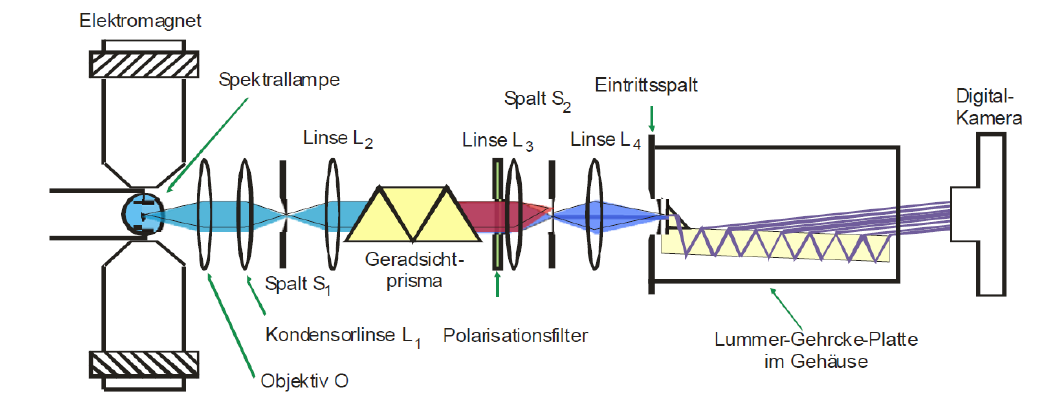
\includegraphics[width=\textwidth]{content/data/aufbau.png}
    \caption{Schematische Darstellung des Versuchaufbaus zum Zeeman-Effekt.} %ref
    \label{fig:aufbau}
\end{figure}

Das Licht der Cd-Lampe wird mit einem Objektiv $O$ und einer Linse $L_1$ scharf auf den Spalt $S_1$ abgebildet.
Anschließend wird mithilfe einer weiteren Linse $L_2$ der Lichtstrahl kollimiert.
Der parallele Lichtstrahl trifft auf das Geradlichtprisma und es können die verschiedenen Spektrallinien beobachtet werden.
\\
Es wird zuerst die blaue Spektrallinie, also der anomale Zeeman-Effekt untersucht.
Dazu wird zuerst mit der Linse $L_3$ ein scharfes Bild auf den Spalt $S_3$ abgebildet und anschließend der Spalt so ausgerichtet, dass ausschließlich die blaue Spektrallinie von der anderen Seite zu sehen ist.
\\
Mit der Linse $L_4$ soll ein scharfes Bild auf die Lummer-Gehrcke-Platte abbgebildet werden.
\\
Nun wird ein Polarisationsfilter hinter das Geradlichtprisma befestigt.
Steht der Polarisator auf $\SI{0}{\degree}$, so wird der Übergang $\Delta m = \pm 1$ bzw. das $\sigma$-polarisierte Licht ausgeblendet.
Hingegen wird bei $\SI{90}{\degree}$ der Übergang $\Delta m = 0$ gefiltert und das $\pi$-polarisiere Licht trifft somit nicht mehr auf die Lummer-Gehrcke-Platte.
\\
Die Ergebnisse werden mit einer auf die Lummer-Gehrcke-Platte gerichteten Digital-Kamera festgehalten.
\\
Erstmal werden die Linien bei ausgeschaltetem Magnetfeld fotografiert.
Anschließend wird das Magnetfeld, soweit es möglich ist (siehe Tab. \ref{tab:magnetfelder}), eingestellt und die Zeeman-Aufspaltung der $\sigma$- und $\pi$-Linien aufgenommen.
\\
Zuletzt wird die rote Spektrallinie untersucht, dazu muss der Spalt angepasst werden.
Anschließend kann das Interferenzmuster bei ausgeschaltetem Magnetfeld aufgenommen werden.
\\
Im nächsten Schritt wird das Magnetfeld eingeschaltet.
Hier ist zu beachten, dass der theoretisch berechnete Wert die maximale Feldstärke übersteigt.
Es wird die maximale Feldstärke verwendet.
Nun wird noch der $\sigma$-Übergang fotografisch festgehalten.